\documentclass[12pt]{article}
\usepackage{times}
\usepackage{amsmath}
\usepackage{a4}
\usepackage{graphicx}
\usepackage{hyperref}

\setlength{\oddsidemargin}{-0.2in}
%\setlength{\evensidemargin}{-0.5in}
\setlength{\textwidth}{6.5in}
\begin{document}
\begin{center}
\Large
\textbf{Numerical Analysis and Programming}\\
\large
Lab Worksheet \#3
\end{center}

The logistic map is defined as 
\[
x_{n+1}=a x_n(1-x_n).
\]
Use \verb!numpy! and \verb!matplotlib! to plot following figures:

\begin{enumerate}
\item Time series plots for $a=3.2$, $3.5$ and $4$ for the first 100 iterations starting from $x=0.1$.  (Fig.~\ref{timeseries})
\item Cobweb plots for $a=3.2$, $3.5$ and $4$ for 50 iterations starting from $x=0.1$. (Fig.~\ref{cobweb})

\item Bifurcation digram. To generate this plot you need to store last half of the $x_i$ points in your time series.  Fig.~\ref{bifurcation} is generated with $\Delta a=0.001$, and 100 iterations for each $a$ value. 

\end{enumerate}
Produce figures as close as possible to the given examples, including legends, labels, ticks, line width, annotation,etc.

\begin{figure}[ht]
\centerline{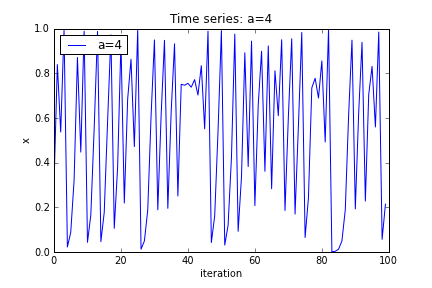
\includegraphics[width=0.6\textwidth]{timeseries_a4.png}}
\caption{Time series plot  for $a=4$.}
\label{timeseries}
\end{figure}

\begin{figure}[h]
\centerline{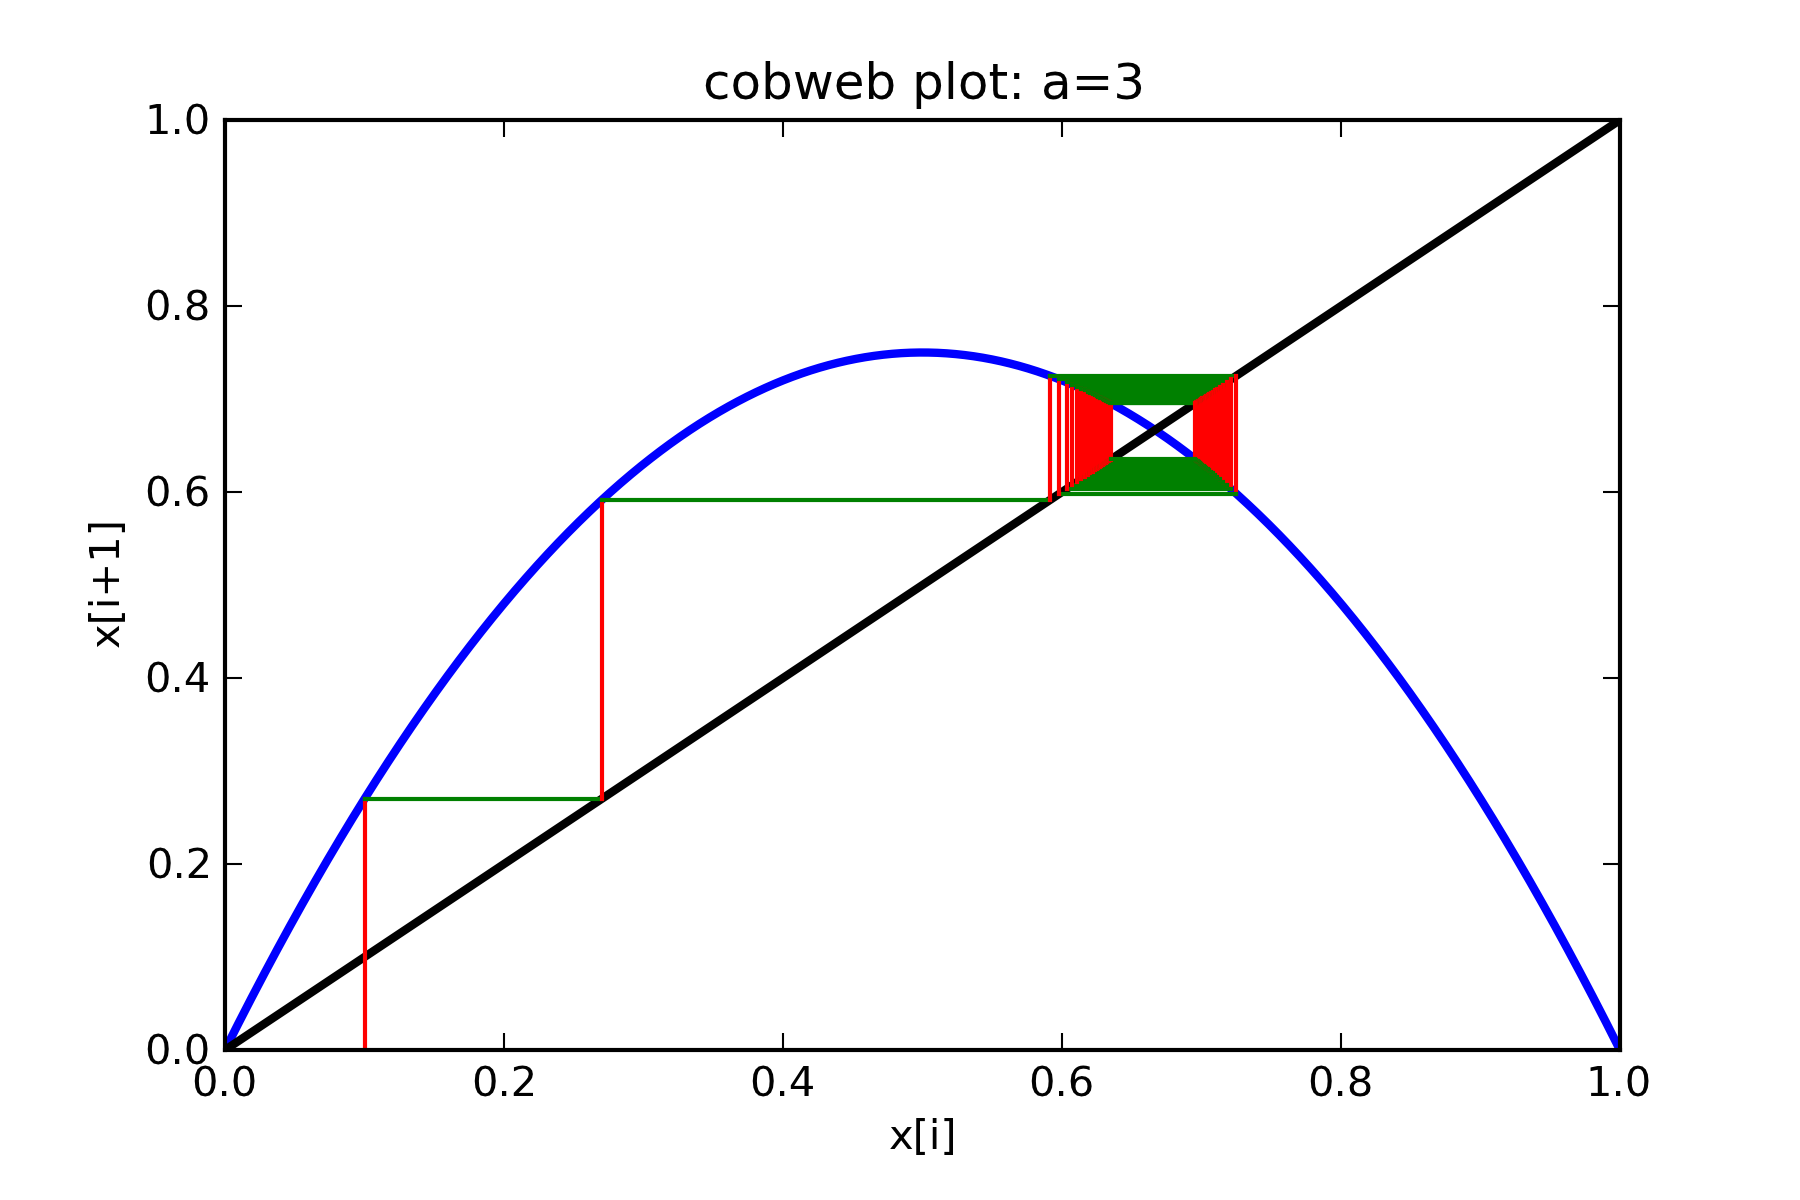
\includegraphics[width=0.6\textwidth]{cobweb_a3.png}}
\caption{Cobweb Plot for $a=3$.}
\label{cobweb}
\end{figure}


\begin{figure}[hb]
\centerline{\includegraphics[width=0.6\textwidth]{bifurcation.png}}
\caption{Bifurcation diagram}
\label{bifurcation}
\end{figure}
\end{document}	
